\documentclass[english,a4paper, 11pt]{article}
\usepackage[T1]{fontenc} %for å bruke æøå
\usepackage[utf8]{inputenc}
\usepackage{graphicx} %for å inkludere grafikk
\usepackage{verbatim} %for å inkludere filer med tegn LaTeX ikke liker
\usepackage{mathpazo}
\usepackage{hyperref}
\usepackage{float}
\usepackage{gensymb}
\usepackage{amsmath}

\title{FYS2150: Magnetisme}
\author{Henrik Haugerud Carlsen}
\date{\today}
\begin{document}

\maketitle

\begin{abstract}
\centering
Often physical systems can be described by linear second-order differential equations, for example the Poisson equation used in electromagnetism. The aim of this report is to rewrite the one-dimensional Poisson equation as a set of linear equations and solve it numerically using algorithms based on the Gaussian elimination method and LU decomposition. The number of FLOPS used by the algorithms and their relative error will be calculated. 
\end{abstract}


\section{Introduction}
The electrostatc potential, $\vec{\phi}$, generated from a localized charge distribution, $\rho(\vec{r})$, in three dimensions can be described by Poissons equation as follows:

\begin{equation}
\nabla^2 \vec{\phi} = -4\pi \rho(\vec{r}).
\label{eq1}
\end{equation}

This can be simplified by utilising the spherical symmetry, which tells us that the potential is constant at at given radius away from the charge distribution independent of change in the polar and/or the asimuttal angle. We can then rewrite the expression to a one-dimensional equation:

\begin{equation}
\frac{1}{r^2} \frac{d}{dr} (r^2\frac{d \vec{\phi}}{dr}) = -4\pi\rho(\vec{r}).
\label{eq2}
\end{equation}

By substituting $\vec{\phi} = \frac{\phi(r)}{r}$, we get:

\begin{equation}
\frac{d^2 \phi}{dr^2} = -4 \pi r \rho(r) \;,
\label{eq3}
\end{equation}

and by letting $\phi \rightarrow u$ and $r \rightarrow x$ we get an expression of the general Poisson equation as

\begin{equation}
-u``(x) = f(x)\;.
\label{eq4}
\end{equation}
Where $x \in (0,1)$.
This can be translated to a set of linear equations. Our problem also contains the boundary conditions $u(0) = u(1) =0$. Discretizing this equation we get the well known expression for the double derivative:

\begin{equation}
-\frac{v_{i+1} + v_{i-1} - 2v_i}{h^2} = f_i \, 
\label{eq5}
\end{equation}
where $i = 1, 2,..., n$.

To be able to use the Gaussian elimination method an LU decomposition to solve the problem we first have to show that the set of linear equations can be rewritten as 

\begin{equation}
A\vec{v} = \vec{b`} \;,
\label{eq6}
\end{equation}
 where A is an $n \times n$ tridiagonal matrix. The elements of $\vec{b`}$ is $b`_i = h^2f_i$. First we start by writing out the expression with $i=1$, getting:
 
 \begin{equation}
 -v_2 + v_0 -2v_i = h^2f_1 = b`_1\;.
 \label{eq7}
 \end{equation}
 Which translates to
 
 \begin{equation}
 -u(2) + u(0) - 2u(1) = h^2f(1)
 \label{eq8}
 \end{equation}
 
Inserting the boundary condition $v(0)= v(1) = 0$ we end up with

\begin{equation}
-u(2) = h^2f(1)\;.
\label{eq9}
\end{equation}
This does not correspond with the matrix A given by the problem set.

 If we do the same for $i=2$ we end up with
 \begin{equation}
 -u(3) -2u(2) = b`-2\;.
 \label{eq10}
 \end{equation}
  
 And for $i = 3$  we get 
 
 \begin{equation}
 -u(4) + u(2) - 2u(3) = h^2f(2)\;,
 \label{eq11}
 \end{equation}
 
 and for $i = 4$ we get
 
 \begin{equation}
 -u(5) + u(3) -2u(4) = h^2f(3)\;,
 \label{eq12}
 \end{equation}
 
 and so on. This leaves us at a general expression for the rows in the matrix as:
 \begin{equation}
 -u(n)  - 2u(n-1) + u(n-2)= b`_n\;.
 \label{eq13}
 \end{equation}
 
 If we insert this for every row in the matrix we end up with a matrix of the from $A\vec{v} = \vec{b`}$.
 
\section{Method}
\subsection{General algorithm}
To solve a set of linear equations of the form $A\vec{v} = \vec{b`}$ an algorithm is developed from the Forward and backward Euler methods. 

$$
    A = \begin{bmatrix}
                           b_1& c_1 & 0 &\dots   & \dots &\dots \\
                           a_1 & b_2 & c_2 &\dots &\dots &\dots \\
                           & a_2 & b_3 & c_3 & \dots & \dots \\
                           & \dots   & \dots &\dots   &\dots & \dots \\
                           &   &  &a_{n-2}  &b_{n-1}& c_{n-1} \\
                           &    &  &   &a_{n-1} & b_n \\
                      \end{bmatrix}\begin{bmatrix}
                           v_1\\
                           v_2\\
                           \dots \\
                          \dots  \\
                          \dots \\
                           v_n\\
                      \end{bmatrix}
  =\begin{bmatrix}
                           f_1\\
                           f_2\\
                           \dots \\
                           \dots \\
                          \dots \\
                           f_n\\
                      \end{bmatrix}.
$$
Our matrix is a tridiagonal one so the first step in the algorithm focuses on making the matrix an upper diagonal matrix, in other words eliminating the elements, $a_i$, below the diagonal. To accomplish this every element $b_i$ has to be mulitiplied by a factor which makes it so that when its is subtracted from the $a_i$ elements the new element is zero. The algorithm is known as the Forward substitution method:

\begin{equation}
b`_i = b_i - \frac{a_{i-1}c_{i-1}}{b`_{i-1}}\;,
\label{Forwardb}
\end{equation}

with the corresponding equation for the updated $f_i$`s:

\begin{equation}
f`_i = f_i - \frac{a_{i-1}f`_{i-1}}{b`_{i-1}}\;.
\label{Forwardf}
\end{equation}
 The updated matrix then becomes an upper triangular matrix:
 
 $$
    A = \begin{bmatrix}
                           b_1& c_1 & 0 &\dots   & \dots &\dots \\
                           0 & b`_2 & c_2 &\dots &\dots &\dots \\
                           & 0& b`_3 & c_3 & \dots & \dots \\
                           & \dots   & \dots &\dots   &\dots & \dots \\
                           &   &  &0  &b`_{n-1}& c_{n-1} \\
                           &    &  &   &0& b`_n \\
                      \end{bmatrix}\begin{bmatrix}
                           v_1\\
                           v_2\\
                           \dots \\
                          \dots  \\
                          \dots \\
                           v_n\\
                      \end{bmatrix}
  =\begin{bmatrix}
                           f_1\\
                           f`_2\\
                           \dots \\
                           \dots \\
                          \dots \\
                           f`_n\\
                      \end{bmatrix}.
$$
Next step is to perform backward substitution which gives us the final diagonal elements:

\begin{equation}
u_i = (f`_i - c_iu_{i+1})/b`_i\;.
\label{Backward}
\end{equation} 

Written i pseudocode this method will look like:

for $i$ in $2,3, ..., n$:
$$
	b`_i = b_i - \frac{a_{i-1}c_{i-1}}{b`_{i-1}}
$$
$$
	f`_i = f_i - \frac{a_{i-1}f`_{i-1}}{b`_{i-1}}
$$
$$
	u_i = \frac{f`_i - c_iu_{i+1}}{b`_i}
$$
This loop ends up using 9n FLOPS.

\subsection{specialized algorithm}

The previous algorithm was made for the general case where knowledge of the elements where more limited. For the case where we know that all the elements $a_i = -1$ and $c_i = -1$ we can write a more effective algorithm to solve the problem. If we write out the calculations we need to find the $b`_i$ elements we get

$$
b`_1 = 2
$$
$$
b`2 = 2-\frac{1}{2} = \frac{3}{2}
$$
$$
b`_3 = 2 - \frac{2}{3} = \frac{4}{3}
$$
$$
b`_4 =  2- 3\frac{3}{4} = \frac{5}{4}
$$
We recognize the pattern as

\begin{equation}
b`_i = \frac{i+1}{i}\;.
\label{Specialb}
\end{equation}

Because we know the constants $a_i$ and $c_i$ the updated values of $f_i$ and $u_i$ becomes:

\begin{equation}
f`_i = f_i + \frac{f_{i-1}}{b_{i-1}}
\label{Specialf}
\end{equation}

\begin{equation}
u_i = \frac{f`_i + u_{i+1}}{b`_i}
\label{Specialu}
\end{equation}

So the pseudocode becomes:

for $i$ in $2,3, ..., n$:

$$
b`_i = \frac{i+1}{i}\;.
$$
$$
f`_i = f_i + \frac{f_{i-1}}{b_{i-1}}
$$
$$
u_i = \frac{f`_i -c_iu_{i+1}}{b`_i}
$$

This method only uses 4N FLOPS, so it the special algorithm is faster than the general one, as expected. 

\subsection{LU decomposition}

We will compare the previously discussed methods with LU decomposition. LU decomposition takes the matrix, $A$, and writes it as a matrixproduct of a lower triangular matrix, $L$, and an upper triangular matrix, $U$. 

$$
    L = \begin{bmatrix}
                           1& 0 & \dots  &\dots   & \dots &\dots \\
                           l_{21} & 1 & 0 &\dots &\dots &\dots \\
                           l_{31}& l_{32}& 1 & 0 & \dots & \dots \\
                           \dots& \dots   & \dots &\dots   &\dots & \dots \\
                           \dots&  \dots &\dots  &\dots &1& 0 \\
                           l_{i1}& \dots   & \dots & \dots  &l_{ij-1}& 1\\
                      \end{bmatrix}
                      $$
                      $$
    	U = \begin{bmatrix}
                           u_{11}& u_{12} & \dots &\dots   & \dots &u_{1j} \\
                           0 & u_{22} & \dots &\dots &\dots &\dots \\
                          \dots & 0& u_{33} & \dots & \dots & \dots \\
                         \dots  & \dots   & \dots &\dots   &\dots & \dots \\
                          \dots &\dots   & \dots &0  &\dots& \dots \\
                           \dots&  \dots  &\dots  &  \dots &0& u_{ij}\\
                      \end{bmatrix}$$
 \newline
The elements can be found by first calculating the elements $u_{1j} = a_{1j}$, then calculating the elements $u_{ij}$, where $i = 2, 3, ..., j-1$, with the following equation:

\begin{equation}
u_{ij} = a_{ij} - \sum_{k=1}^{i-1} l_{ik}u_{kj}\;.
\label{LUu}
\end{equation}

Then find the diagonal elements from

\begin{equation}
u_{jj} = a_{jj} - \sum_{k=1}^{j-1} l_{jk}u_{kj}\;.
\label{LUdiagonal}
\end{equation}

Lastly calculate the remaining elements:

\begin{equation}
l_{ij} = \frac{1}{u_{jj}}(a_{ij} - \sum_{k=1}^{i-1}l_{ik}u_{kj}\;.
\label{LUl}
\end{equation}

When this is done the decomposed system can be solved by first solving $L\vec{z} = \vec{f}$, then solving $U\vec{x} = \vec{z}$. Here we set $U\vec{x} = \vec{z}$. What we end up with is a system which can be solved by $for$ loops without more decomposition.

The LU decomposition program used in this paper is taken from






\section{Results}

Using both our general and specialized algorithm we can compute the numerical solution to our matrix equation. This was done for $n$ that ranged from $n = 10^1$ up to $n = 10^7$. Here the resulting plots for $n = 10, 10^3$ and $10^5$ is shown. That gives the plots

\begin{figure}[h]
\centering
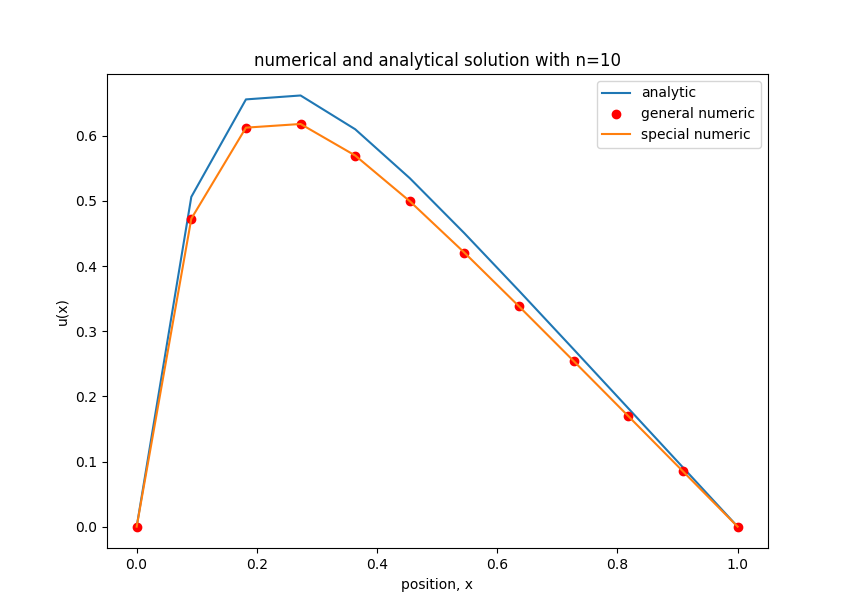
\includegraphics[scale=0.5]{poisson_n1.png}
\caption{analytical, general and specialized solution to the poisson equation for $n = 10^1$}\label{fig1}
\end{figure}

\begin{figure}[h]
\centering
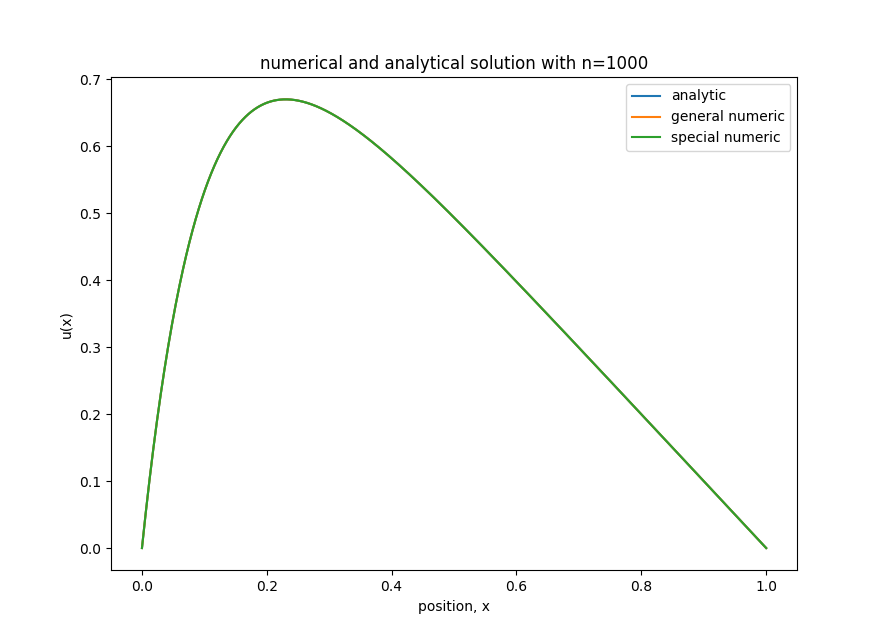
\includegraphics[scale=0.5]{poisson_n3.png}
\caption{analytical, general and specialized solution to the poisson equation for $n = 10^3$}\label{fig2}
\end{figure}

\begin{figure}[h]
\centering
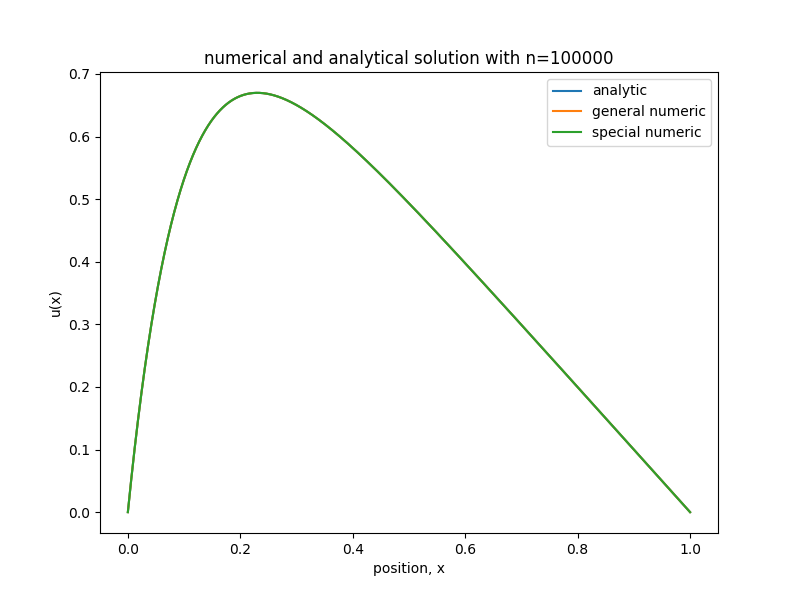
\includegraphics[scale=0.5]{poisson_n5.png}
\caption{analytical, general and specialized solution to the poisson equation for $n = 10^5$}\label{fig3}
\end{figure}

At the same time we computed the relative error of the specialized algorithm against the analytical solution to our problem so we could get a relation between the max relative error of the calculations and the steplengths, $h$. This was found using equation \ref{eq?} and by plotting the maximum error of each steplength as a function of the briggsian logarithm of $h$ we got the plot 

\begin{figure}[h]
\centering
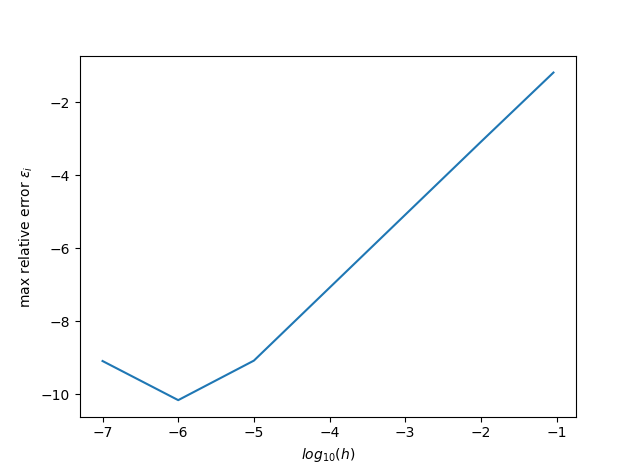
\includegraphics[scale=0.5]{max_rel_error.png}
\caption{the max relative error plotted as a function of $log_{10}(h)$}\label{fig4}
\end{figure}

the time spent computing the numerical solution was found, there was also used a even more general LU decomposition algorithm to compare the time spent. The time spent is presented in a tabular form

\begin{table}[h]
\caption{time spent for general, specialized and LU decomposition for the different $n$}\label{tab1}\center
\begin{tabular}{|c|c|c|c|}
\hline
n & General (s) & Specialized (s) & LU decomp. (s) \\
\hline
$10^1$ & $<1\cdot10^{-4}$ & $<1\cdot10^{-4}$ & $<1\cdot10^{-3}$ \\
\hline
$10^2$ & $1\cdot10^{-3}$ & $<1\cdot10^{-3}$ & 0.14 \\
\hline
$10^3$ & $5\cdot10^{-3}$ & $4\cdot10^{-3}$ & 154 \\
\hline
$10^4$ & $5.7\cdot10^{-2}$ & $1.7\cdot10^{-2}$ & -\\
\hline
$10^5$ & $3.9\cdot10^{-1}$ & $1.9\cdot10^{-1}$ & - \\
\hline
$10^6$ & 3.4 & 1.6 & -\\
\hline
$10^7$ & 31.8 & 15.5 & -\\
\hline
\end{tabular}
\end{table}

\section{References}


\end{document}

